\documentclass{standalone}

% tikz
\usepackage{tikz}
\usetikzlibrary{positioning,fit,shapes,decorations.pathreplacing}

% colors
\definecolor{Prism3}{RGB}{41, 174, 128}


% boxes for tikz
\newcommand{\rbox}[3]{
    \node(#1)[
        draw,
        line width=1pt,
        rounded corners,
        %text width=30pt,
        minimum height=30pt,
        %text centered,
        align=center,
        fill=white,
        #2
    ]{#3};
}

\newcommand{\grbox}[3]{
    \node(#1)[
        draw,
        line width=1pt,
        color=lightgray,
        rounded corners,
        %text width=30pt,
        minimum height=30pt,
        %text centered,
        align=center,
        fill=white,
        #2
    ]{#3};
}

\newcommand{\group}[4]{
    \node(#1)[
        draw,
        %dashed,
        %thick,
        line width=0.8pt,
        densely dotted,
        rounded corners,
        inner xsep=10pt,
        inner ysep=15pt,
        %text centered,
        yshift=5pt,
        fit=(#2)(#3),
        %label={[left=2cm]#4}
    ](#1){};s
    \node[below right, inner xsep=14pt, inner ysep=5pt] at (#1.north west) {#4};
}
\begin{document}
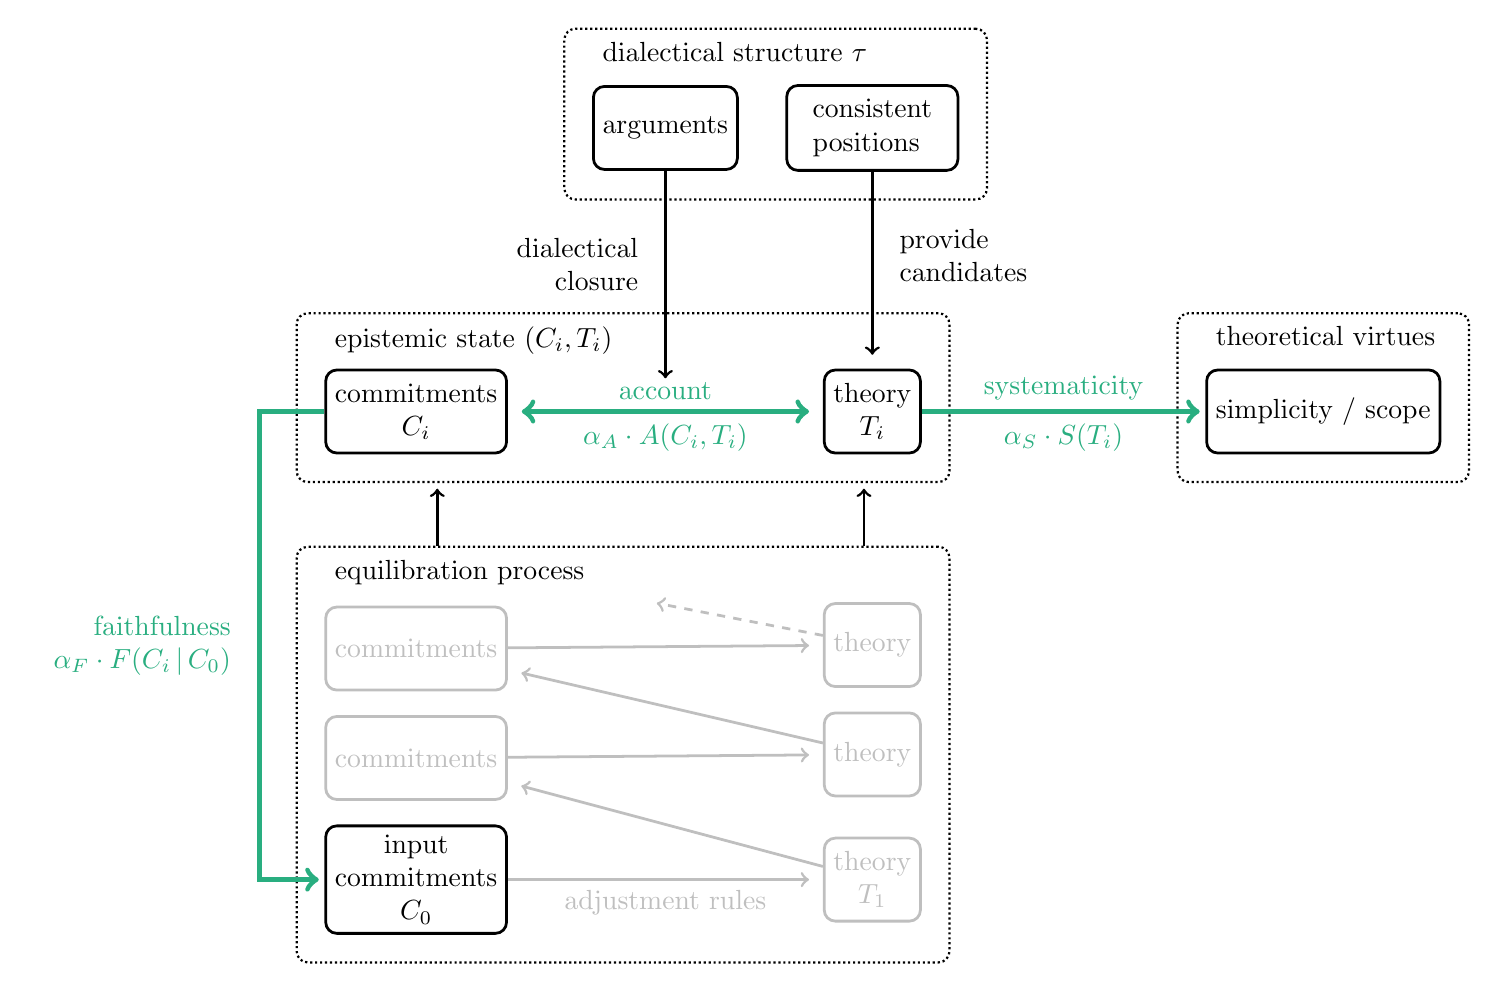
\begin{tikzpicture}
	\rbox{RE coms}{}{commitments\\$C_{i}$}
	\rbox{RE the}{right=4cm of RE coms} {theory\\$T_{i}$}
	
	\draw[<->, line width=2pt, shorten >=5pt, shorten <=5pt, color=Prism3] (RE coms) -- (RE the) node[midway, below] (fit) { $\alpha_{A}\cdot A(C_{i}, T_{i})$} node[midway, above] (account) {account};
	
	\group{RE pos}{RE coms}{RE the}{epistemic state $(C_{i}, T_{i})$}
	
	\rbox{bgthe}{above=2.5cm of RE the} {\begin{tabular}{l}
	   consistent\\
	   positions   
	\end{tabular}}
	
	\rbox{bginf}{at={(fit |- bgthe)}} {arguments}
	
	\draw[->, line width=1pt, shorten >=5pt] (bgthe) -- (RE the)
	node[pos=0.44, right] (supp) {\begin{tabular}{l}
	   provide\\
	   candidates   
	\end{tabular}};
	
	\draw[->, line width=1pt, shorten >=12pt] (bginf) -- (fit)
	node[pos=0.4, left] (infit) {\begin{tabular}{r}
	     dialectical\\
	     closure 
	\end{tabular}};
	
	\group{bg}{bginf}{bgthe}{dialectical structure $\tau$ }
	
	\rbox{epgoals}{right=3.6cm of RE the}{simplicity / scope}
	
	\group{ep}{epgoals}{epgoals}{theoretical virtues}
	
	\draw[->, line width=2pt, shorten >=2pt, color=Prism3] (RE the) -- (epgoals)
	node[pos=0.5, below] (just) {$\alpha_{S}\cdot S(T_{i})$} node[pos=0.5, above] (sys) {systematicity};
	
	\node (in) [below=4.7cm of RE coms] {};
	
	\rbox{inbox}{below=4.7cm of RE coms}{input\\ commitments\\$C_{0}$}

	\grbox{com1}{above=0.3cm of inbox}{commitments}
	\grbox{the1}{at={(RE the |- inbox)}}{theory\\$T_{1}$}
	
	\grbox{com2}{above=0.3cm of com1}{commitments}
	\grbox{the2}{above=0.5cm of the1}{theory}
	
	\grbox{the3}{above=0.3cm of the2}{theory}
	
	\draw[->, line width=1pt, color=lightgray, shorten >=5pt] (inbox) -- (the1)
	node[midway, below, color=lightgray] (adj1) {adjustment rules};
	\draw[->, line width=1pt, color=lightgray, shorten >=5pt] (the1) -- (com1);
	\draw[->, line width=1pt, color=lightgray, shorten >=5pt] (com1) -- (the2);
	\draw[->, line width=1pt, color=lightgray, shorten >=5pt] (the2) -- (com2);
	\draw[->, line width=1pt, color=lightgray, shorten >=5pt] (com2) -- (the3);
	\node(help)[above=0.5cm of com2]{};
	\draw[->, dashed, line width=1pt, color=lightgray, shorten >=85pt] (the3) -- (help);
	
	\group{process}{inbox}{the3}{equilibration process}
	
	\draw[->,
	line width= 1pt,
	shorten >= 2pt] ([xshift=1.8cm]process.north west) -- ([xshift=1.8cm]RE pos.south west);
	
	\draw[->,
	line width= 1pt,
	shorten >= 2pt] ([xshift=-1.1cm]process.north east) -- ([xshift=-1.1cm]RE pos.south east);
	
	\node (1) [left=0.7cm of RE coms] {};
 
 	\draw[line width=2pt, color=Prism3, shorten >=-1pt] (RE coms) -- (1.center);
	\draw[->, line width=2pt, shorten >=2pt, color=Prism3] (1.center)  |- (inbox) node[pos=0.25, left] (resp) {\begin{tabular}{r}
	     faithfulness\\
	     $\alpha_{F}\cdot F(C_{i}\,\vert\, C_{0})$ 
	\end{tabular}};
\end{tikzpicture}
\end{document}